\begin{tabular}{cccc}
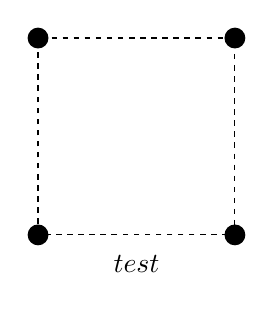
\begin{tikzpicture}[x=2.5cm,y=2.5cm]
\draw[dash pattern=on 2pt off 2pt] (0,0) rectangle (1,1);
\draw [fill=black,line width=1.5pt] (0,0) circle (3pt);
%node_label%\draw (0,0) node {<++>};
\draw [fill=black,line width=1.5pt] (1,0) circle (3pt);
%node_label%\draw (1,0) node {<++>};
\draw [fill=black,line width=1.5pt] (0,1) circle (3pt);
%node_label%\draw (0,1) node {<++>};
\draw [fill=black,line width=1.5pt] (1,1) circle (3pt);
%node_label%\draw (1,1) node {<++>};

%cursor

\draw (0.5,-0.15) node {$test$};

\end{tikzpicture}
%%%
&
%%%
\end{tabular}